% Chapter Template

\chapter{Future Work} % Main chapter title

\label{Chapter8} % Change X to a consecutive number; for referencing this chapter elsewhere, use \ref{ChapterX}

\lhead{Chapter 8. \emph{Future Work}} % Change X to a consecutive number; this is for the header on each page - perhaps a shortened title

%----------------------------------------------------------------------------------------
%	SECTION 1
%----------------------------------------------------------------------------------------

\section{What Comes Next?}
The experiments layed out in the previous chapters have shown that \ac{MRL} using \acp{MAE} allows for the unsupervised learning of a grounded representation of images and language. How then, can this be used to improve robotic technologies?

I see many potential applications for \ac{MRL} within the field of \ac{HRI}. \autoref{fig:fsm} shows an example of how the \ac{MAE} can be included in a robotic system.


\begin{figure}
\centering
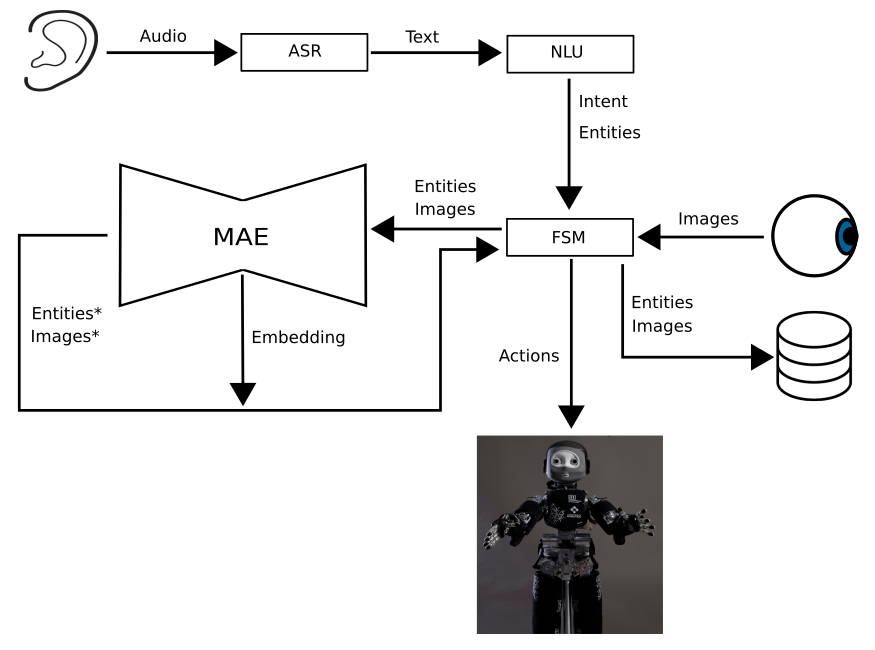
\includegraphics[width=\textwidth]{Figs/futureWork/fsm.png}
\caption{An example of how the \ac{MAE} can be used as part of a robotic system.}
\label{fig:fsm}
\end{figure}

Consider the scenario of a human interacting with a robot to teach it a set of objects and their visual attributes as well as the words used to describe the objects and their visual attributes. In a laboratory setting it is feasable to have only a single object in view at any given time. This is not true for real world scenarios. However, with the introduction of a \ac{FSM} controlled via a \ac{NLU} module, it is simple to use a \ac{MAE} trained with \ac{MRL} to discern which object is being referred to by the human. This is demonstrated in \autoref{fig:disamb}

\begin{figure}
\centering
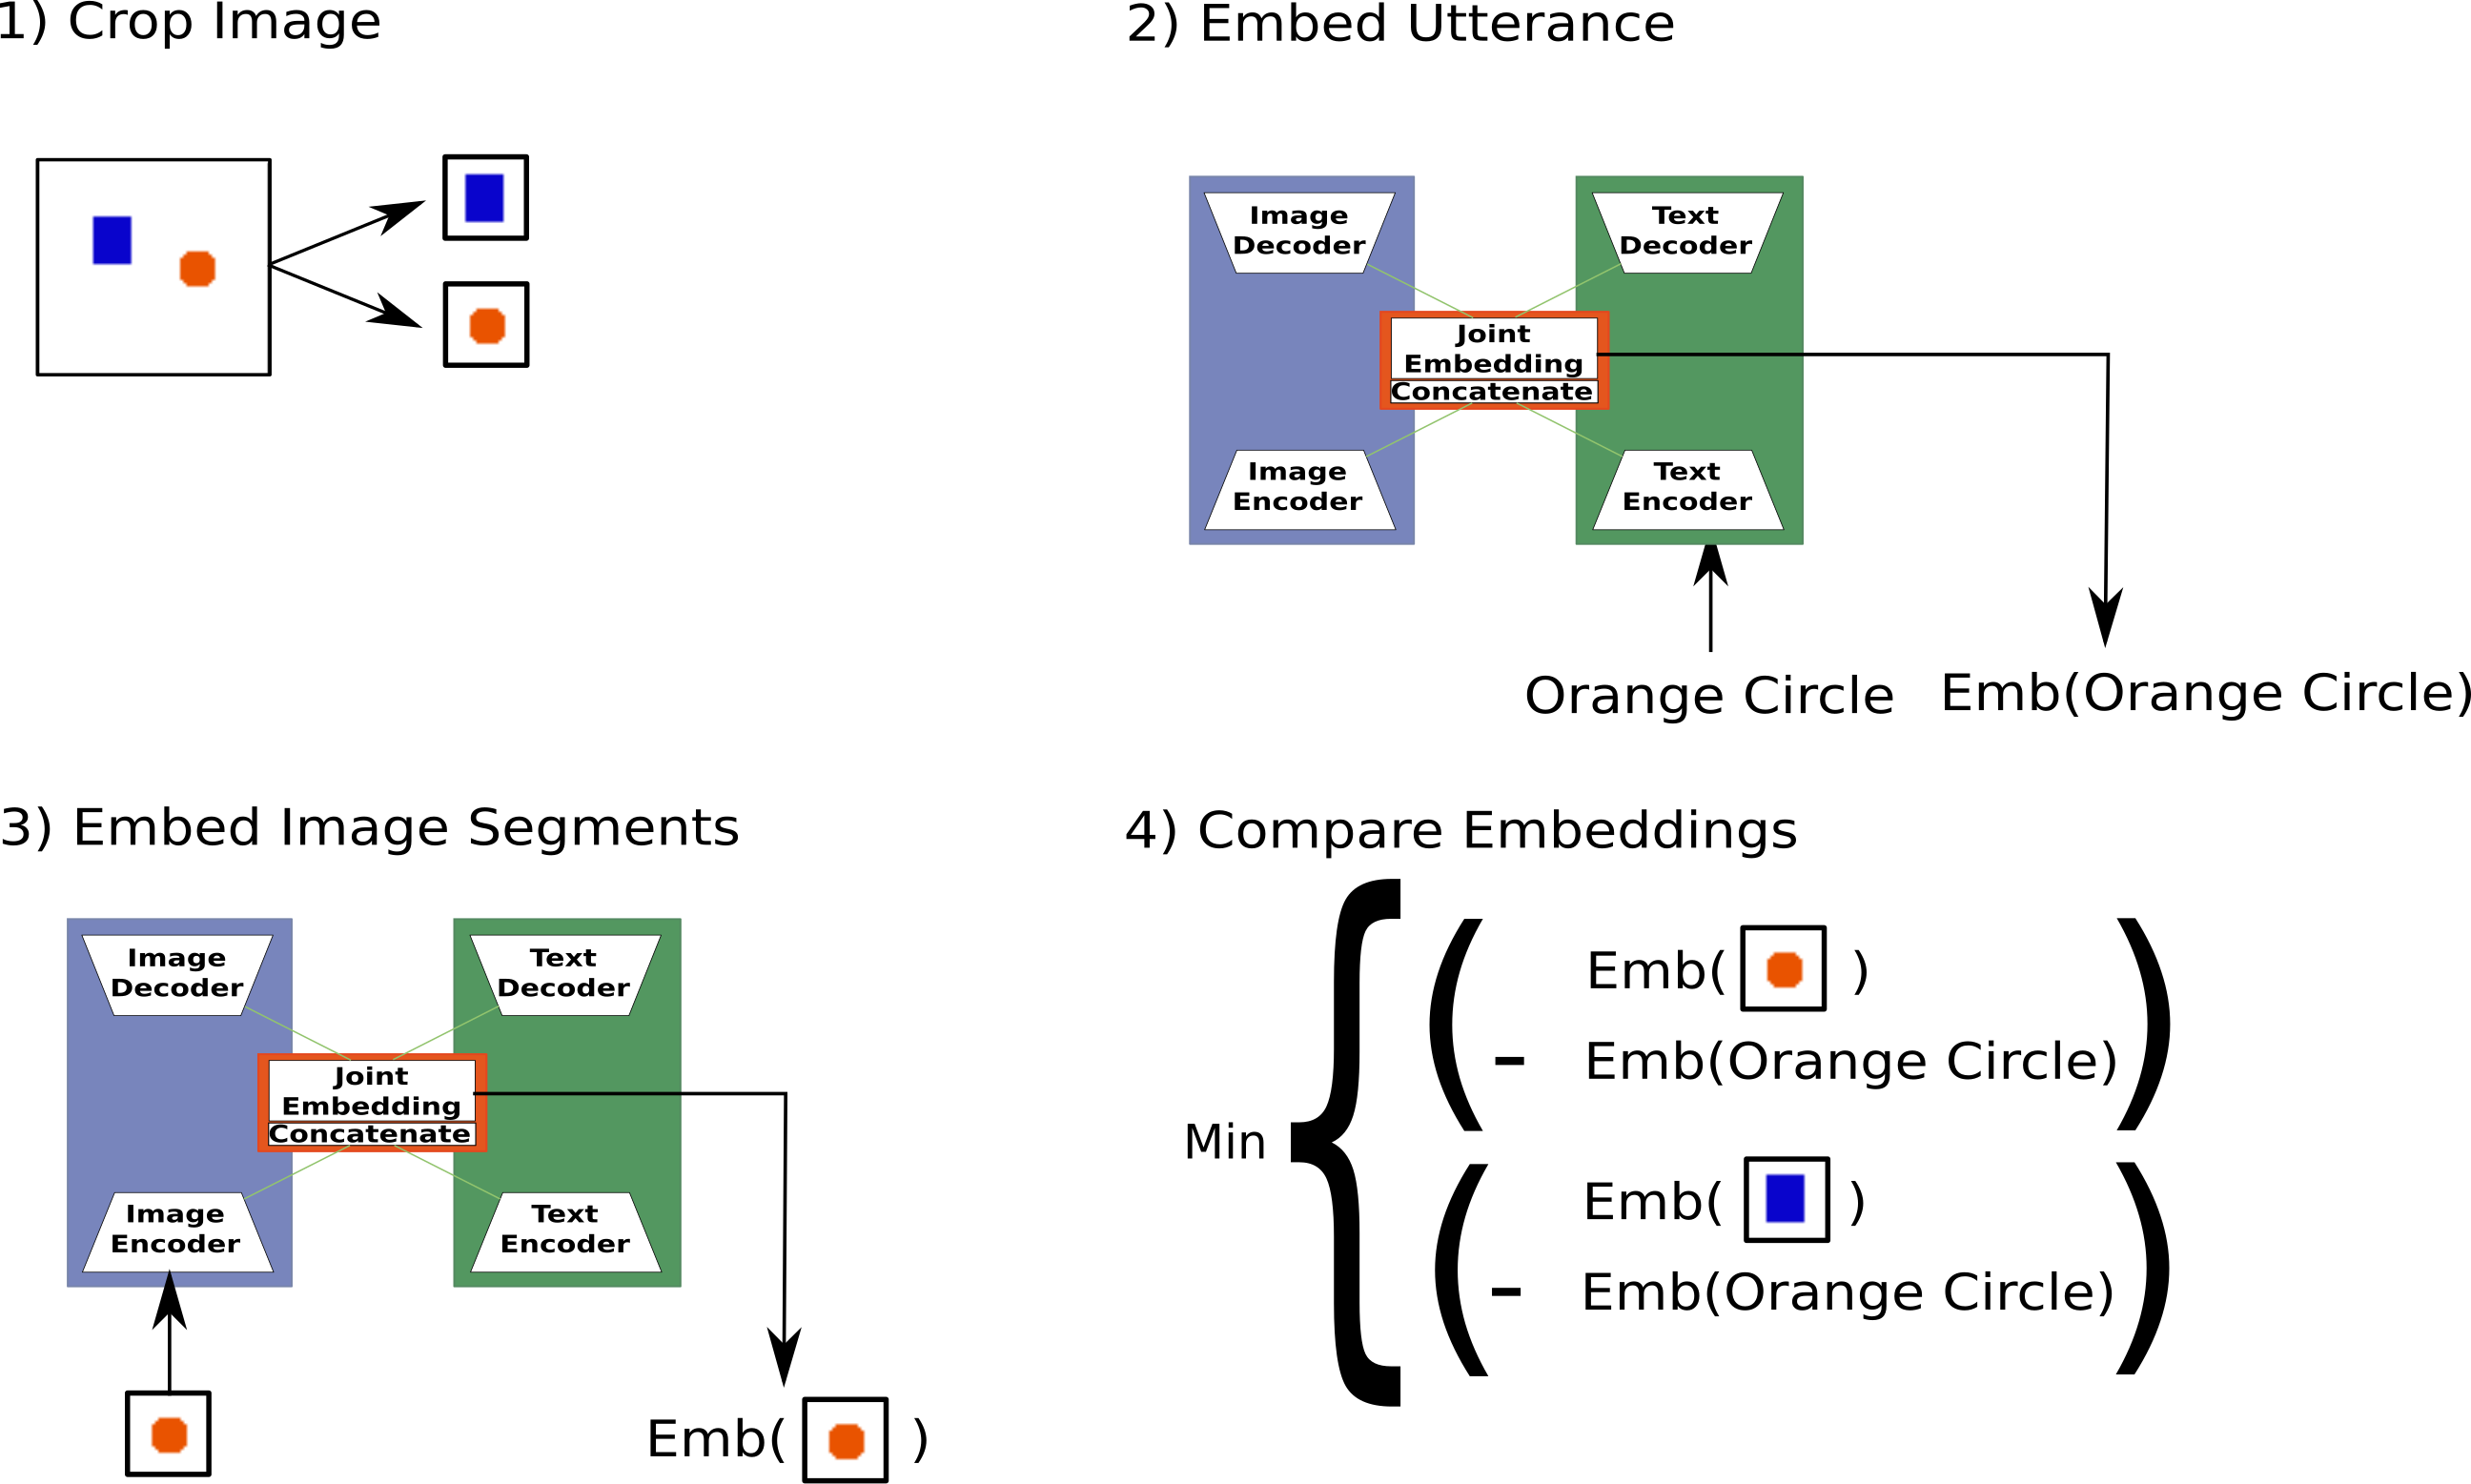
\includegraphics[width=\textwidth]{Figs/shapes/findingRefferant.png}
\caption{An example of using an MAE trained with MRL to disambiguate which object is being referred to in a scene.}
\label{fig:disamb}
\end{figure}

First, the image is split into patches, this can be done naively by sliding a window over the image and processing each patch. However this is not very computationally efficient and is likely to give ambiguous results, depending on the stride of the window, as multiple image patches may contain parts of the object of interest. Therefore it would be sensible to make use of an object detector such as Yolo v3 \cite{redmon2018yolov3} to predict object bounding boxes.

Comparing the embedding of each image patch to the embedding of the query, the image patch of interest should have the smallest \ac{MSE} between it and the query.

In order for the scenario depicted in \ref{fig:disamb}, an \ac{NLU} module must be trained to extract the Intent of the human's utterance as well as any Entities which the human refers to. Fortunately, these types of \acp{NLU} are easily built using open source libraries like Rasa \cite{rasa}.



Developing the infrastructure for this type of scenario would allow for the exploration of questions such as:

\begin{itemize}
\item How many training examples does the \ac{MAE} require to operate accurately?
\item Is their an upper limit on the number of objects, visual attributes and words which the \ac{MAE} can learn?
\item How does regenerating a missing modality affect classification accuracy? Can the embedding of the regnerated missing modality be exploited to enhance  multimodal recognition techniques?
\end{itemize}

I believe \ac{MRL} can be used as a general tool for facilitating \ac{HRI} experiments, with the \ac{MAE} providing a piece of a cognitive architecture which translates low level sensory percepts (vision) to high level symbols (language).


%-----------------------------------
%	SUBSECTION 1
%-----------------------------------
